\documentclass{homework}
% \usepackage{graphicx} % Required for inserting images
\usepackage{amsmath}
\usepackage{gensymb}
\usepackage{subfig}
\usepackage{float}

\class{ECEN 5478}
\title{Homework Set 2}
\author{Sean Jennings}
\date{September 21, 2023}

\begin{document}
\maketitle

Assume all citations to theorems, lemmas, etc. refer to Beck unless otherwise 
noted.

\newcommand{\dist}{\text{Dist}}
\section{Problem 1}
\begin{letterenum}
    \item The given set $S = \{x \in \R^n: \alpha \leq a^T x \leq \beta\}$ where $a \in \R^n$ and $\alpha, \beta \in \R$
        is the intersection of two half-spaces:
        \begin{equation}
            S = \{x \in \R^n: a^T x \leq \beta\} \cap
                 \{x \in \R^n: (-a^T) x \leq -\alpha\}
        \end{equation}
        Since hyperplanes are convex (Lemma 6.3) and the intersection of
        convex sets are complex (Lemma 6.6), $S$ is convex.

    \item The convexity of the given set follows by the same reasoning as
        part (a).

    \item Fix $a = \mat{a_1 & 0}^T, c = \mat{c_1 & 0}^T \in R^2$ for
        any $a_1, c_1, r \in \R$ s.t. $r > a_1 > 0$ and $c_1 = r - a_1$.


        Let $S$ and $T$ be the balls $\mathcal{B}(-c, r)$ and
            $\mathcal{B}(c, r)$, respectively and let $C(S, T)$ denote
            the set of points closer to $S$ than to $T$.

        Figure (\ref{fig:balls}) provides a visaulization of the counter
        example.
        \begin{center}
            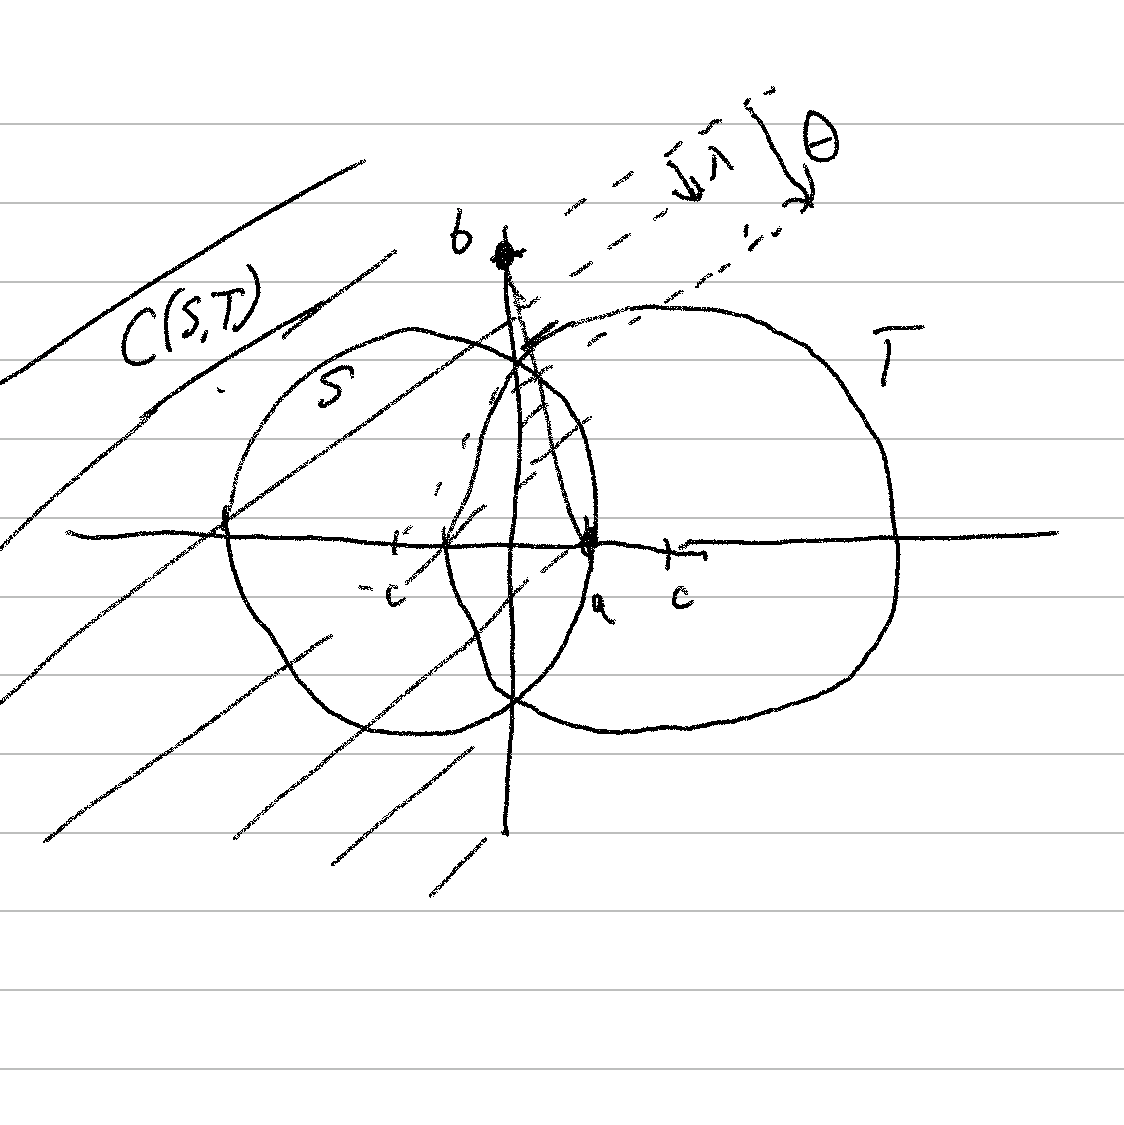
\includegraphics[width=0.8\linewidth]{balls.png}
            \captionof{figure}{Visualization of counter example}
            \label{fig:balls}
        \end{center}
        
        We take note that the distance of a point $x \in R^2$ to a ball
        with center $c\in\R^2$ and $r$ is given by:
        \begin{equation}
            \dist(x, \mathcal{B}(c, r)) = \biggl(
                \begin{array}{ll}
                    \norm{x - c} - r &\qquad \text{ if } \norm{x - c} > r \\
                    0 &\qquad \text{ otherwise}
                \end{array}
            \biggr.
        .
        \end{equation}

        If we take the right open half phane minus $S$,
        $H = \{x \in \R^2: -\epsilon_1^T x < 0\} \setminus S$
        (where $\epsilon_1$ denotes the first member of the canonical basis),
        then for any $x=\mat{x_1 & x_2}^T \in H$, we take
        \begin{align}
            (\dist(x, T) + r)^2 &\leq \mnorm{x_1 - c_1 \\ x_2}^2 \\
                &= (x_1 - c_1)^2 + x_2^2 \\
                &= x_1^2 - 2x_1c_1 + c_1^2 + x_2^2 \\
                &< x_1^2 + 2x_1c_1 + c_1^2 + x_2^2 \\
                &= \mnorm{x_1 + c_1 \\ x_2}^2 \\
                &= (\dist(x, S) + r)^2
        \end{align}
        so that $\dist(x, T) < \dist(x, S)$ and $x \notin C(S, T)$.
        Thus, $H \subset C(S, T)^c$. ($A^c$ denotes the complement of set $A$.)

        Fix $b \in \{x \in \R^2: -\epsilon_1^T x = 0\} \setminus S\cup T$.

        Now, we check that both $a$ and $b$ are in $C(S, T)$, before checking
        the points between them for convexity. $\dist(a, S) = 0$ so $a\in$ 
        $\dist(b, S) = \dist(b, T)$, since
        \begin{equation}
            \norm{b - (-c)} = \mnorm{c_1 \\ b_2}
                = \mnorm{-c_1 \\ b_2} = \norm{b - c}.
        \end{equation}
        So also $b\in C(S, T)$.

        Finally, let $z: [0, 1] \to \R^2$ be the map:
        \begin{equation}
            z(\lambda) = \lambda a + (1 - \lambda)b =
                \mat{\lambda a_1 \\ (1-\lambda) b_2}
        \end{equation}
        Then, $z(1) = \norm{b - c} < r < \norm{a - c} = z(0)$ so that by
        I.V.T., there exists $\theta \in [0, 1]$ s.t. $\norm{z(\theta) - (-c)} = r$
        since $z$ is continuous. Then, for any $\lambda \in (0, \theta)$,
        the following hold:
        \begin{letterenum}
            \item $\norm{z(\lambda - (-c)) > r}$, and
            \item $\lambda a_1 > 0$ implies $-\epsilon_1^T z(\lambda) \leq 0$
        \end{letterenum}
        So $z(\lambda) \in H \subset C(S,T)^c$ and thus $C(S,T)$ does not
        satisfy conditions for convexity.

    \item The author will continue contemplating this exercise.


\end{letterenum}

\section{Problem 2}
Note:
"cont. diff." is used as shorthand for "continuously differentiable".
"s.t." = "such that"
\begin{letterenum}
    \item $f$ is twice cont. diff. so we can check the hessian:
    \begin{equation}
        \nabla^2 f(x) = \begin{bmatrix}
            2 & 0 \\ 0 & 2
        \end{bmatrix} \succeq 0,
    \end{equation}
    where $\succeq 0$ denotes the matrix is positive semidefinite. Since the
    hessian is positive semidefinite, $f$ is convex.

    \item Since $C = \{x\in\R^2: x_1\geq0, x_2\geq0\}$ is not open, we must
        use the gradient inequality to check convexity.
        Let $x = \mat{0 & 1}^T$, $y = \mat{1 & 0}^T$.
        We observe the gradient of $f$ is
        \begin{equation}
            \nabla f(x) = \mat{x_2 \\ x_1}
        \end{equation}
        which so that
        \begin{equation}
            f(x) + \nabla(x)^T (y-x) = \mat{1 & 0} \mat{1 \\ -1} = 1 > 0 = f(y).
        \end{equation}
        Thus, by the gradient inequality, f is not convex.

    \item Since $C = \{x\in\R^n: x_1 > 0, x_2>0\}$ is open, and $f$ is twice
    cont. diff., second order methods apply. The hessian is
    \begin{equation}
        \nabla^2 f(x) = \mat{
            2x_1^{-3}x_2 & (x_1x_2)^{-2} \\
            (x_1x_2)^{-2} &  2x_2^{-3}x_2
        } = (x_1x_2)^{-1}\mat{
            2x_1^{-2} & (x_1x_2)^{-1} \\
            (x_1x_2)^{-1} & 2x_2^{-2}
        } = 
    \end{equation}
    Let $A\in\R^{n \times n}$ be the matrix in the second equality
    s.t. $\nabla^2 f(x) = (x_1x_2)^{-1} A$. Since $(x_1x_2)^{-1} > 0$,
    $A \succeq 0$ implies $\nabla^2 f(x) \succeq 0$.

    Since $A$ is a 2x2 matrix, if $\text{Tr}(A) \geq 0$ and $\det(A) > 0$ then 
    $A \succeq 0$, by Prop. 2.20. Since also $x_1^{-2} > 0$ and $x_2^{-2} > 0$,
    we have
    \begin{align}
        \text{Tr}(A) &= 2(x_1^{-2} + x_2^{-2}) > 0 \\
        \det(A) &= 4(x_1x_2)^{-2} - (x_1x_2)^{-2} = 3 (x_1x_2)^{-2} > 0
    \end{align}
    Therefore, $\nabla^2 f(x) \succeq 0$ for all $x \in C$, and $f$ is convex
    over $C$.

    \item It was proven in lecture that the sum of $k$ functions
    $f(x) = f_1(x) + f_2(x), \dots, f_k(x)$, where $f, f_i: \R^n \to \R$ and $f_i$ is convex
    for each $i = 1,\dots,k$, is also convex.

    Let $f(x) = f_1(x) + f_2(x)$ where $f_1 = \norm{\cdot}$ and
    $f_2(x) = e^{-(x_1 + x_2)}$. As shown in example 7.4 (and also follows
    easily from the triangular inequality), the norm is convex. So it remains
    to show that $f_2$ is convex.

    $f_2$ is twice cont. diff. and we are considering a domain of $\R^2$ so 
    the second-order characterization of convexity holds. The Hessian of $f_2$
    is
    \begin{equation}
        \nabla^2 f_2(x) = e^{-(x_1 + x_2)} \mat{1 & 1 \\ 1 & 1}.
    \end{equation}
    Since the 2x2 matrix of ones has eigenvalues $\lambda_{1,2} = 0,2$
    and $e^{-(x_1 + x_2)} > 0$ for all $x = \mat{x_1 & x_2}^T \in \R^2$,
    we have $\nabla^2 f_2(x) \psd$. Thus, $f$ is convex.
\end{letterenum}

\section{Problem 3 (More perturbed contractions)}

We will write $x_k^* := x^*(w_k)$.

The desired bound is given by:
\begin{align}
    \norm{x_k - x_k^*} &= \norm{F(x_{k-1}, w_k) - x_k^*} \\
        &\leq \norm{F(x_{k-1}, w_k) - F(x_{k-1}^*, w_k)}
            + \norm{F(x_{k-1}^*, w_k) - F(x_k^*, w_k)} \\
        &\leq \ell_x \norm{x_{k-1} - x_{k-1}^*}
            + \ell_x \norm{x_{k-1}^* - x_k^*} \\
        &\leq \ell_x \norm{x_{k-1} - x_{k-1}^*}
            + \ell_x \biggl(
                \frac{\ell_w}{1 - \ell_x} \norm{w_k - w_{k-1}}
            \biggr).
\end{align}
Now we iterate to find the bound in terms of initial values:
\begin{align}
    \norm{x_k - x_k^*} &\leq \ell_x^k \norm{x_0 - x_0^*}
            + \frac{\ell_x \ell_w}{1 - \ell_x} \biggl(
                \sum_{i=0}^{k-1} \ell_x^i
            \biggr) \sup_{\tau \geq 0} \norm{w_{\tau + 1} - w_\tau} \\
        &\leq \ell_x^k \norm{x_0 - x_0^*}
        + \frac{\ell_x \ell_w}{(1 - \ell_x)^2}
            \sup_{\tau \geq 0} \norm{w_{\tau + 1} - w_\tau}.
\end{align}

Since we are given that $\{w_k\}_{k\in\N}$ is generated by the contracting
linear map $w_{k+1} = Aw_k$ with $\norm{A} < 1$, we can compute more specific
bounds. For any $k\geq0$, we have
\begin{equation}
    \norm{w_{k+1}} = \norm{Aw_k} \leq \norm{A}\norm{w_k} < \norm{w_k}
\end{equation}
and therefore the norm of $w_k$ is decreasing monotonically so that
$\norm{w_0} > \norm{w_k}$ for all $k>0$.

Noting that $\norm{A - I} \leq \norm{A} + \norm{I} < 2$, we derive
the following inequality relation for the suprenum:
\begin{equation}
    \sup_{\tau \geq 0} \norm{w_{\tau + 1} - w_\tau}
        = \sup_{\tau\geq0} \norm{(A - I)w_\tau} < 2 \norm{w_0}
\end{equation}

\section{Problem 4}
Let $F: \R^n \to \R^n$ be the Picard iterator for the sequence $\{x_k\}$
s.t. $F(x) = Ax + b$. Then, $f$ is a contraction since it has contraction
factor $\ell = \norm{A} < 1$.

Proof: We compare the distance between two points $x,y \in \R^n$ before
and after an iteration:

\begin{align}
    \frac{\norm{F(x) - F(y)}}{\norm{x - y}} &=
            \frac{\norm{(Ax + b) - (Ay + b)}}{\norm{x - y}} \\
        &= \frac{\norm{A(x-y)}}{\norm{x - y}} \\
        &\leq \frac{\norm{A}\norm{x-y}}{\norm{x - y}} \\
        &= \norm{A} = \ell.
\end{align}

By the Banach Contraction Theorem, the following hold
\begin{letterenum}
    \item A fixed point $x^*$ exists and is unique, and
    \item the sequence $\{x_k\}$ converges to $x^*$ for all initial conditions.
\end{letterenum}

\end{document}
